\graphicspath{{\currfiledir/images/}}

\chapter{Conceitos Introdutórios}

%=====================================================

Este capítulo introduz, brevemente, os conceitos básicos de grafos que serão utilizados ao longo dessa dissertação. Os conceitos apresentados neste capítulo podem ser acessados nas seguintes bibliografias: \cite{bondymurty1976}; \cite{west2002}; \cite{bondymurty2008}; \cite{feofiloff2018}.


\section{Teoria de grafos}
Muitas situações do mundo real podem ser convenientemente descritas por meio de um diagrama que consiste em um conjunto de pontos, juntamente com linhas que unem certos pares destes pontos \cite{bondymurty1976}. Por exemplo, os pontos podem representar pessoas, com linhas unindo pares de amigos ou os pontos podem ser centros de comunicação, com linhas representando links de comunicação. Tais diagramas buscam saber se dois pontos dados são unidos por uma linha, a maneira pela qual eles são unidos é irrelevante. Uma abstração matemática de situações desse tipo dá origem ao conceito de grafos \cite{bondymurty2008}.

\begin{definition}
    Um grafo $G$ é denotado por um par ordenado $(V(G), E(G))$, onde $V(G)$ é um conjunto de vértices e $E(G)$ é um conjunto de ligações entre pares de vértices de $G$, chamados de arestas. São denotadas por $n = |V(G)|$ e $m = |E(G)|$ as cardinalidades dos conjuntos $V(G)$ e $E(G)$, respectivamente.
\end{definition}


\section{Representação visual}
Os grafos têm esse nome porque podem ser representados graficamente. Cada vértice é indicado por um ponto e cada aresta por uma linha que une os pontos que representam suas extremidades \cite{bondymurty1976}.

Existem diversas maneiras de representação para um grafo. Os pontos (vértices) e conexões (arestas) são meramente um modelo visual da estrutura de dados, isto é, não têm significado.

A seguir, dois exemplos de representações de dois grafos, $G$ e $H$.

\begin{example}
    Considere o grafo $G$, Figura~\ref{sec2:ex-repr-grafo-G}, onde
    \begin{center}
        $V(G) = {u, v, w, x, y}$
    \end{center}
    \begin{center}
        $E(G) = {a, b, c, d, e, f, g, h}$
    \end{center}
\end{example}

\begin{example}
    Considere o grafo $H$, Figura~\ref{sec2:ex-repr-grafo-H}, onde
    \begin{center}
        $V(H) = {v_0, v_1, v_2, v_3, v_4, v_5}$
    \end{center}
    \begin{center}
        $E(H) = {e_1, e_2, e_3, e_4, e_5, e_6, e_7, e_8, e_9, e_10}$
    \end{center}
\end{example}

\begin{figure}[!htb]
    \centering
    \begin{subfigure}{.5\textwidth}
        \centering
        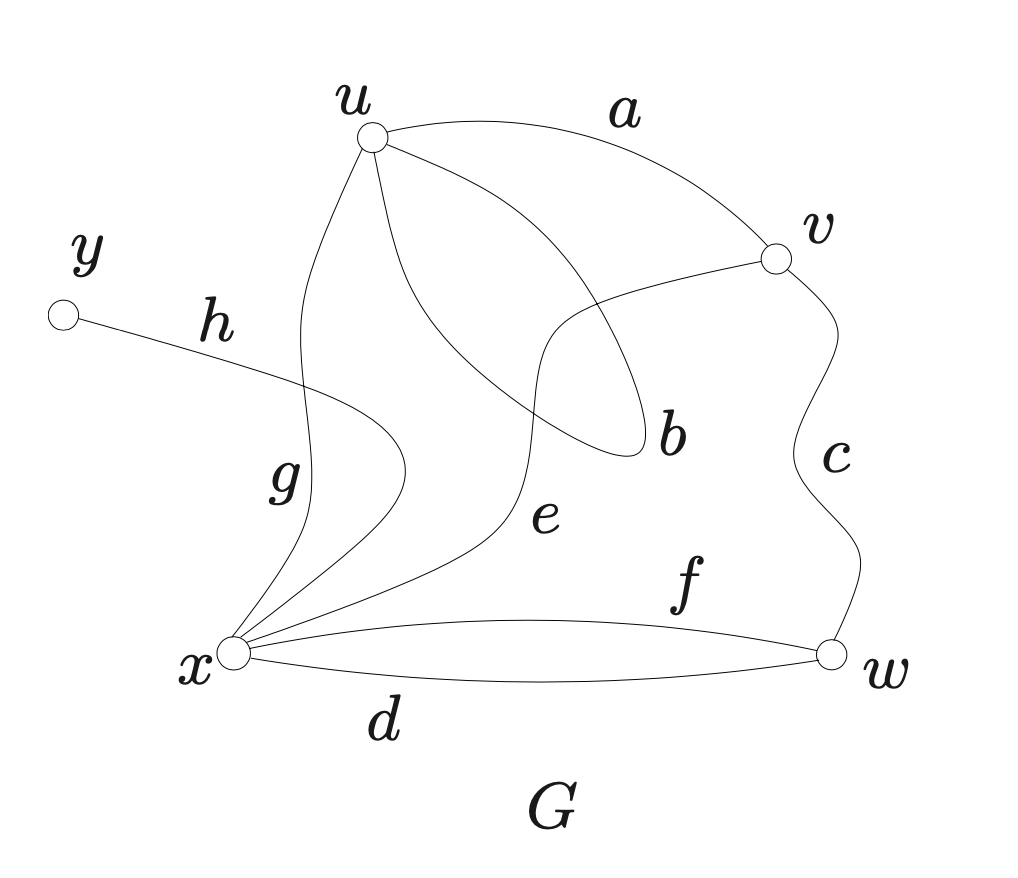
\includegraphics[scale=0.4]{representacao-grafo-G.png}
        \caption{$G$.}
        \label{sec2:ex-repr-grafo-G}
    \end{subfigure}%
    \begin{subfigure}{.5\textwidth}
        \centering
        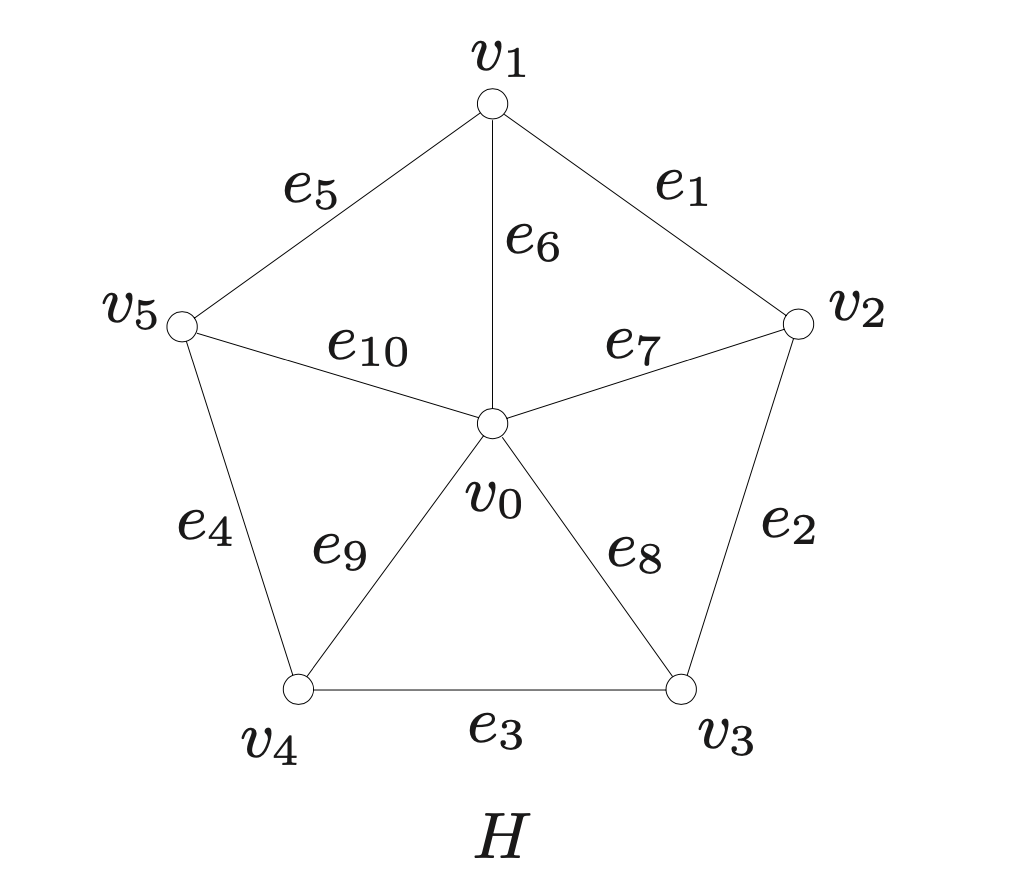
\includegraphics[scale=0.4]{representacao-grafo-H.png}
        \caption{$H$.}
        \label{sec2:ex-repr-grafo-H}
    \end{subfigure}
    \caption{Representação visual de grafos.}
    \label{sec2:ex-repr-grafo-G-H}
\end{figure}


\section{Grau de vértices e número de arestas}
O número de arestas incidentes a um vértice introduz o conceito de grau de um vértice. Algumas bibliografias ainda subdividem este conceito em definições de leques de entrada e saída, ou seja, o grau do leque de saída de um vértice se dá pelas arestas que "saem do vértice" e, de forma intuitiva, o grau de um vértice de entrada é o número de arestas que incidem em um vértice, "entram no vértice". De forma complementar, percebe-se que a soma dos graus de saída de todos os vértices de um grafo é igual ao número de arestas do grafo. A soma dos graus de entrada de todos os vértices também é igual ao número de arestas. Segue daí que um grafo com V vértices tem no máximo \begin{math}V (V - 1)\end{math} arestas. Esse número é apenas um pouco menor que ${V}^2$.

\begin{definition}
    Dado um grafo $G = (V(G), E(G))$, o grau de um vértice $v$, denotado por $d(v)$, é o número total de arestas de $G$, incidentes a $v$.
\end{definition}


\section{Direcionamento}
Usando-se das definições anteriores, nesta seção iremos explanar umas das principais propriedades da conectividade de grafos (relacionamento entre vértices de um grafo $G$). Os grafos podem ou não ser direcionados, pondo-se em exemplos reais, a relação de amizade em um rede social por exemplo, pode ser denotada como não direcionada, pois um amigo $a$ é amigo de $b$, assim como o inverso. Já em rotas e trajetos (mapas), as ruas possuem direcionamento, isto é, para um exemplo em que uma rua possui mão única, a relação do ponto de interseção de seu início e fim pode ser dado como de $a$ para $b$, porém não o inverso, pois seria considerado contramão.

Considere a Figura~\ref{sec2:ex-grafo-nao-direcionado}. Este é um exemplos de um grafo $G$, não direcionado, onde $V(G) = \left\{a, b, c, d\right\} $ e $E(G) = \left\{\left\{a, b\right\}, \left\{a, c\right\}, \left\{a, d\right\}, \left\{b, c\right\}, \left\{b, d\right\}, \left\{c, d\right\}\right\}$. Nota-se que as arestas $\left\{a, b\right\} $ e $\left\{b, a\right\} $ são considerados redundantes, motivo pela qual o conjunto $E(G)$ apresenta somente uma delas.

\begin{figure}[!htb]
    \centering
    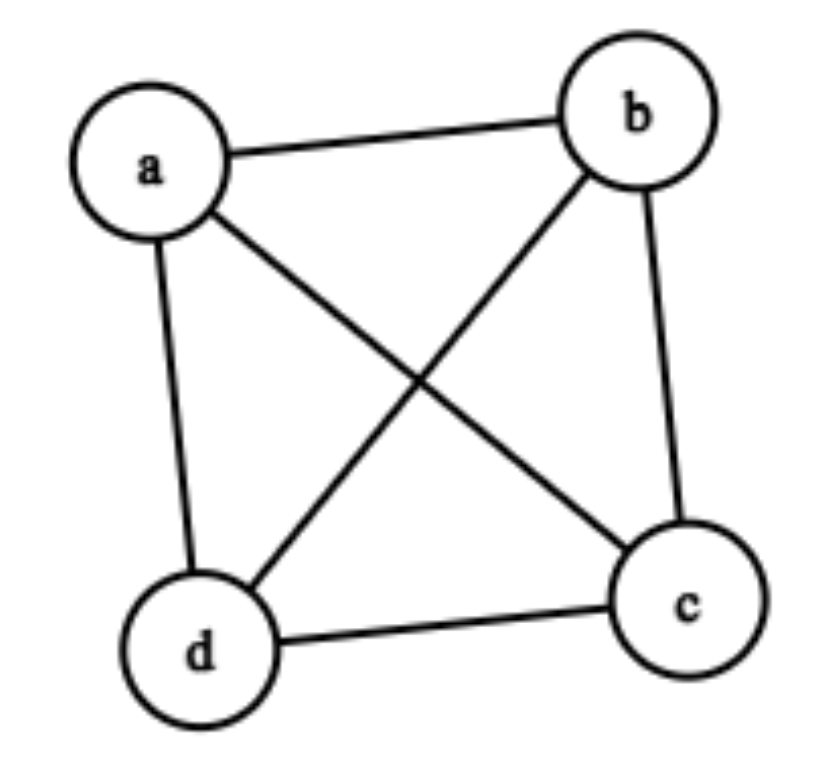
\includegraphics[scale=0.3]{grafo-nao-direcionado.png}
    \caption{Grafo não direcionado.}
    \label{sec2:ex-grafo-nao-direcionado}
\end{figure}

Considere a Figura~\ref{sec2:ex-grafo-direcionado}. Este é um exemplos de um grafo $G$, direcionado, onde $V(G) = \left\{a, b, c, d\right\} $ e $E(G) = \left\{ab, ad, bc, ca, db\right\} $. A aresta $ab$, indica que há uma relação de $a$ para $b$ e o inverso não é verdade.

\begin{figure}
    \centering
    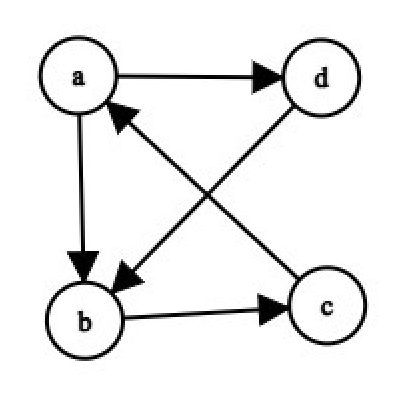
\includegraphics[scale=0.65]{grafo-direcionado.png}
    \caption{Grafo direcionado.}
    \label{sec2:ex-grafo-direcionado}
\end{figure}


\section{Subgrafos e supergrafos}
Dado um grafo $G$, um subgrafo de $G$ é um grafo com todos os seus pontos e retas em $G$. Se $G'$, é um subgrafo de $G$, então $G$ é um supergrafo de $G'$. Um subgrafo de extensão é um subgrafo, contendo todos os pontos de $G$. Para qualquer conjunto $S$ de pontos de $G$, o subgrafo induzido $<S>$ é o subgrafo máximo de $G$ com conjunto de pontos $S$. Desta forma, dois pontos de $S$ são adjacentes em $<S>$, se e somente se, eles são adjacentes em $G$.

Na Figura~\ref{sec2:grafo-subgrafo}, $G''$ é um subgrafo de extensão de $G$, mas $G'$ não é; $G'$, é um subgrafo induzido, mas $G''$ não é \cite{harary1994}.

\begin{figure}[!htb]
    \centering
    \begin{subfigure}{.3\textwidth}
        \centering
        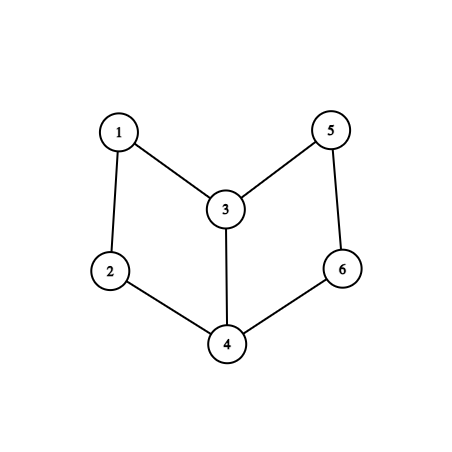
\includegraphics[scale=0.3]{sub-sup-grafo-G.png}
        \caption{$G$.}
        \label{sec2:grafo-G}
    \end{subfigure}%
    \begin{subfigure}{.3\textwidth}
        \centering
        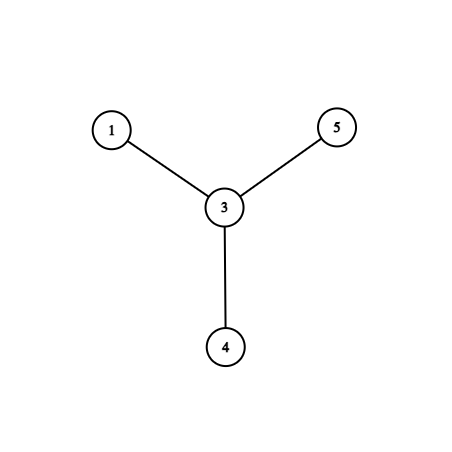
\includegraphics[scale=0.3]{grafo-G'.png}
        \caption{$G'$.}
        \label{sec2:grafo-G'}
    \end{subfigure}%
    \begin{subfigure}{.3\textwidth}
        \centering
        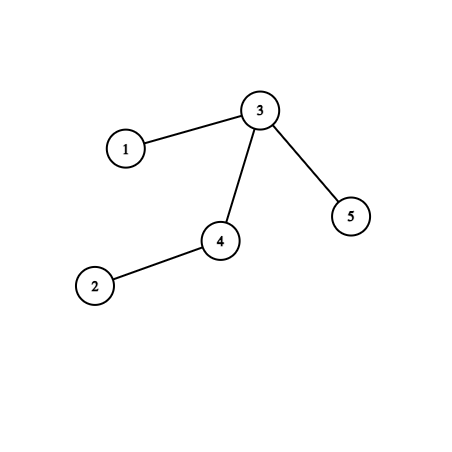
\includegraphics[scale=0.3]{grafo-G''.png}
        \caption{$G''$.}
        \label{sec2:grafo-G''}
    \end{subfigure}
    \caption{Um grafo e dois subgrafos.}
    \label{sec2:grafo-subgrafo}
\end{figure}

\begin{definition}
    Um grafo $H$ é um subgrafo de $G$, escrito como $H\subseteq G$ se $V(H) \subseteq V(G)$ e $E(H) \subseteq E(G)$.
\end{definition}


\section{Passeios (\emph{walk}), caminhos (\emph{path}) e ciclos}
Previamente, foram definidos alguns princípios básicos dos grafos, vértices e arestas. Considerando os princípios até agora apresentados, esta seção visa definir as noções de passeios e caminhos em um grafo.

Um passeio (\emph{walk}) em um grafo é uma sequência de vértices dotada da seguinte propriedade: se $v$ e $w$ são vértices consecutivos na sequência, então $v - w$ é uma aresta do grafo (note que o inverso de um passeio não é, em geral, um passeio). Uma aresta do passeio é qualquer aresta $v - w$ do grafo tal que $w$ é o sucessor de $v$ no passeio. Um passeio é fechado (\emph{closed}) se tem pelo menos duas arestas e seu primeiro vértice coincide com o último.

Um caminho (\emph{path}) em um grafo é um passeio sem arestas repetidas, ou seja, um passeio em que as arestas são todas diferentes entre si. Um caminho é \emph{simples} se não tem vértices repetidos. Por exemplo, $0 - 2 - 7 - 3 - 6$ é um caminho simples no grafo $G$ da Figura~\ref{sec2:walk-path-def}.

\begin{figure}
    \centering
    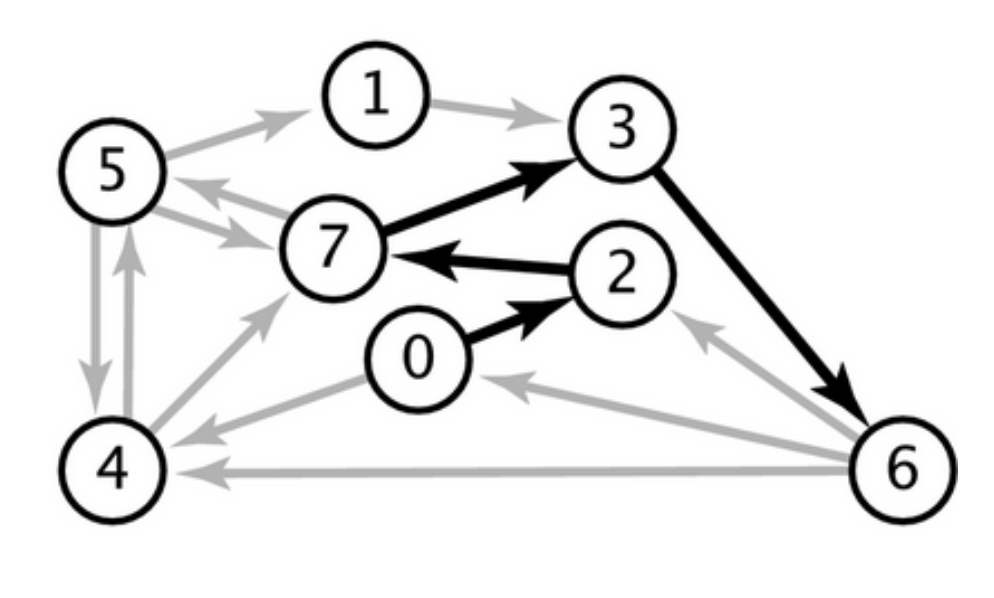
\includegraphics[scale=0.5]{walk-path-def.png}
    \caption{Um grafo direcionado com 8 vértices.}
    \label{sec2:walk-path-def}
\end{figure}

Todas as arestas de um caminho apontam na mesma direção de um vértice para o seu sucessor. Há quem goste de enfatizar esse fato dizendo caminho dirigido em vez de caminho.

A origem de um caminho é o seu primeiro vértice. O término é o seu último vértice. Se um caminho tem origem $s$ e término $t$, dizemos que vai de $s$ a $t$. O comprimento de um caminho é o número de arestas do caminho. Se um caminho tem $n$ vértices, seu comprimento é pelo menos \begin{math}n - 1\end{math}; se o caminho é simples, seu comprimento é exatamente \begin{math}n - 1\end{math} \cite{feofiloff2018}.

Tendo-se das definições acima, um ciclo em um grafo nada mais é que um caminho fechado, ou seja, tem comprimento maior que 1, sem arestas repetidas.

\begin{definition}
    Dado um grafo $G = (V(G), E(G))$, um passeio $P = (v_1, ..., v_k)$ em $G$ é uma sequência de vértices de $G$, tal que, para todo par consecutivo de vértices $(v_i - 1, v_i)$, com $2 \leq i \leq k$, temos que $v_i - 1v_i$ é uma aresta de $G$. Se não houverem vértices repetidos em $P$, dizemos que $P$  é um caminho. Um ciclo no grafo $G$ é uma sequência de vértices $C = (v_1,v_2,...,v_k)$ se $P = (v_1, ..., v_k)$ é um caminho em $G$ e $v_1v_k \in E(G)$.
\end{definition}


\section{Árvores e florestas}
Em grafos, uma árvore é um grafo conexo sem ciclos. Uma floresta é um grafo com cada componente conectado em uma árvore. Uma folha em uma árvore é qualquer vértice de grau 1. A Figura~\ref{sec2:tree-forest-def} apresenta uma árvore e uma floresta com duas árvores.

\begin{figure}
    \centering
    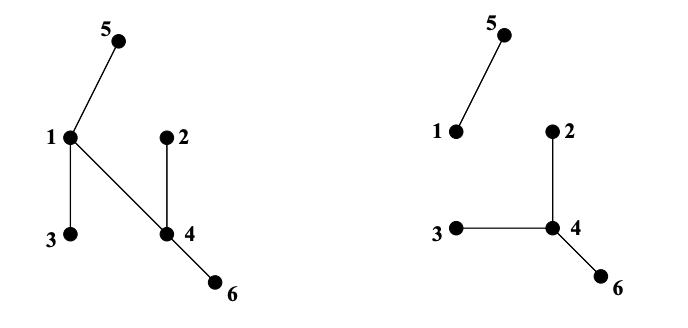
\includegraphics[scale=0.7]{tree-forest-def.png}
    \caption{Um grafo e uma floresta com duas árvores.}
    \label{sec2:tree-forest-def}
\end{figure}

%=====================================================
